\chapter{Preliminary tools: units, vectors, calculus, Newton's laws}

\section{Measurements and measure units}
In physics (as in any science), each time we want to express the result of a measurement we must always specify its \textit{measure unit}, i.e. a standard quantity to refer to when quoting a result; in setting the standard of measure units, the \textit{International System of Units} (or SI) helps us, defining seven fundamental units for the corresponding physical quantities

\begin{table}[htbp]
\begin{center}
\begin{tabular}{|c|c|c|} \hline
\textbf{Quantity} & \textbf{Unit(name)} & \textbf{Unit(symbol)} \\ \hline
Length & meter & m \\ \hline
Time & second & s \\ \hline
Mass & kilogram & kg \\ \hline
Temperature & kelvin & K \\ \hline
Electric current & ampere & A \\ \hline
Amount of substance & mole & mol \\ \hline
Luminous intensity & candle & cd \\ \hline
\end{tabular}
\end{center}
\caption{A list of the SI measure units}
\end{table}

\noindent From these, we can build countless derived measure units, and what follows are just some examples; for the purpose of this class, we want to quote for convenience some other standard units derived from these, that we will make use of frequently
\begin{table}[htbp]
\begin{center}
\begin{tabular}{|c|c|c|c|} \hline
\textbf{Name} & \textbf{Comments} & \textbf{Symbol} & \textbf{Approximate value} \\ \hline
Speed of light &Einstein's pride & $c$ & $3\cdot 10^8$m/s \\ \hline
Light year &$c\,\,\times$ 1\,year& ly & 9.5$\cdot10^{15}$m\\ \hline
Hubble constant &Fundamental quantity in cosmology&$H_0$&$10^{-10}$yr$^{-1}$\\ \hline
Parsec &Cosmological length scale& pc & 3ly \\ \hline
Hubble horizon &Size of the observable universe today& $d_H$&3Gpc\\ \hline 
Solar mass & Mass of the sun & $M_\odot$ & 2$\cdot10^{30}$ kg\\ \hline
CMB temperature &Observed temperature of the background radiation&$T_{CMB}$&2.78 K \\ \hline 

\end{tabular}
\end{center}
\caption{Some useful quantities that occur frequently in Cosmology}
\end{table}

\section{Organizing physical quantities: scalars, vectors and tensors}
Cosmology, as a part of physics, is a scientific theory that is formulated in terms of precise mathematical terms; these concepts help exemplify the reasonments, which would be much complicated if tried to be explained in terms of pure words, and help develop the same reasonments more naturally. In this section, we want to introduce the basic mathematical framework with which physical quantities are usually described. We saw before that any physical quantity is associated with its proper measure unit; there is more: we distinguish physical quantities in three main categories, namely \textit{scalars}, \textit{vectors} and \textit{tensors}. 
\subsection{Scalars}
We give the name \textit{scalar} to all physical quantities that can be completely characterized by only one number; for example, when we talk about the mass of a body, or a planet, or a star, we know that this mass can be completely described by only one number, with its measure unit. For example, the mass of the sun is given by $M_\odot\approx 2\cdot 10^{30}$\,kg. We can try to push this definition a little bit further, saying that a \textit{scalar} is a quantity that is \textit{invariant} (i.e. does not change) under rotations. Thinking about the sun, we can safely say in fact that its mass certainly does not depend on the direction we look at it (invariance under rotations). 
\subsection{Vectors}
Not all the quantities in physics are scalars: for example, when we need to describe a body that moves (it can be the earth orbiting the sun), we need to specify a number that describes the magnitude of its velocity $v$, but that's not all, cause to completely characterize its velocity we also need to specify its \textit{direction}. This can be done specifying the three numbers $\mathbf{v}=(v_x,v_y,v_z)$, which are the components of the velocity $\mathbf{v}$ along the three axes $x,y,z$. This quantity $\mathbf{v}$, that carries information on the direction of the motion is called a \textit{vector}, and can be indicated in bold, $\mathbf{v}$, or with the notation $v_i$, with the index $i$ being one between $x,y,z$ or $1,2,3$. Let's examine what happens under rotations: we cannot say anymore that the components $v_i$ are invariant under rotations, because if we rotate our $(x,y,z)$ axes, the components will change as well. When we perform an axes' rotation the velocity components (and in general any vector 
components) will change from $v_i$ to $v'_i$ with
\begin{equation}
v'_i=\sum_{j=1}^3R_{ij}v_j
\end{equation}
Being $R_{ij}$ an appropriate matrix of real numbers; each quantity that transforms in such a way (only involving linear terms, not $v^2,v^3,...$) is called a \textit{vector}. If we are provided two vectors $\mathbf{a},\mathbf{b}$, we can easily build a scalar $s$ out of them with the following operation called \textit{scalar product}
\begin{equation}
\label{scalarprod}
s=\mathbf{a}\cdot\mathbf{b}\equiv \sum_{i=1}^3a_ib_i
\end{equation}
This quantity $s$ so defined is a true scalar, in the sense that it's invariant under rotations; think about the following examples
\begin{itemize}
\item Let a body move with velocity $\mathbf{v}$; the magnitude of its velocity $v=\sqrt{\mathbf{v}\cdot{\mathbf{v}}}$ is obviously rotation invariant
\item Let a body move with velocity $\mathbf{v}$ and another body move with velocity $\mathbf{u}$; their directions of motion form an angle $\theta$ given by
\begin{equation}
\cos{\theta}=\frac{\mathbf{v}\cdot\mathbf{u}}{vu}
\end{equation}
which is clearly rotation invariant
\end{itemize}
\subsection{Tensors}
The natural extension of the concept of vector, considering rotation properties, is that of \textit{tensor}: if a vector is a triplet of numbers $v_i$ that transforms under a rotation $\mathbf{R}$ in the way
\begin{equation}
v'_i=\sum_{j=1}^3R_{ij}v_j
\end{equation} 
we can define a \textit{tensor} (with two indices) $T_{ij}$ ($i,j=1,2,3$) as an object that transforms not with one but two $\mathbf{R}$ matrices
\begin{equation}
T'_{ij}=\sum_{l,m=1}^3R_{il}R_{jm}T_{lm}\equiv R_{il}R_{jm}T_{lm}
\end{equation}
Where the last $\equiv$ means that we adopted a particular convention where if an index appears twice, we must sum over all possible values of that index (example sum over $m=1,2,3$ and $l=1,2,3$). We can easily generalize this definition to tensors with more than two indices; as an invitation, keep in mind that these concepts are really useful to describe spacetime and gravity in the Einstein's way. For example the metric of the spacetime, that describes its geometry, is a tensor with two indices (usually denoted with $g_{\mu\nu}$) while the Riemann tensor, which describes the curvature of spacetime, is a tensor with four indices (usually denoted with $R_{\mu\nu\rho\sigma}$) with $\mu,\nu,\rho,\sigma=0,1,2,3$ with the added 0-th component as time. 

\section{A little bit of calculus}
The reason for introducing calculus tools and techniques in physics and cosmology, is that usually physical quantities, let them be scalars (temperature, density,...), vectors (velocity, gravitational field, ...) or tensors (metric, curvature,...), are usually space and time dependent. We then need an efficient mathematical tool to understand how these quantities \textit{change} in space and time; we introduce then the concepts of \textit{derivative} and \textit{integral}. 
\subsection{Derivatives}
Let be $\mathbf{x}=(x,y,z)$ be a generic point in space and $f(\mathbf{x})$ \textit{any} physical quantity (can be scalar, vector or tensor) that depends on the position where we are in space (it can be the temperature of the air in a room, the velocity of the water on the sea, the curvature of space due to a planet, etc). Since in general $f(\mathbf{x}_1)\neq f(\mathbf{x}_2)$, we want to quantify how different are these two quantities. We usually do that computing the difference $f(\mathbf{x}_1)-f(\mathbf{x}_2)$, and this gives us an idea on how big is the difference between $f$ in two different positions; the concept of \textit{derivative} is simply the expression of this concept but when the two points $\mathbf{x}_1,\mathbf{x}_2$ are really close to each other $\mathbf{x}_1\approx\mathbf{x}_2$. In this case we can approximate 
\begin{equation}
f(\mathbf{x}_1)-f(\mathbf{x}_2)\approx \nabla f(\mathbf{x}_1)\cdot(\mathbf{x}_1-\mathbf{x}_2)
\end{equation}
Where $\nabla f(\mathbf{x})$ is called \textit{derivative} or \textit{gradient} of the quantity $f$ at the point $\mathbf{x}$ and expresses the \textit{rate of change} of $f$ at $\mathbf{x}$
\subsubsection{Note 1}
If instead of space, our quantity $f$ depends on time $t$, the definition is even simpler, but in this case we use the notation
\begin{equation}
f(t_1)-f(t_2)\approx f'(t_1)(t_1-t_2)
\end{equation}
Where we indicated the derivative at $t_1$ as $f'(t_1)$; to make the previous approximate relation more exact, we can take into account that also the derivative $f'$ varies on time, and construct a \textit{second derivative} $(f')'\equiv f''$. It is claimed that any (well behaved) quantity can be approximated as 
\begin{equation}
f(t_1)-f(t_2)=f'(t_1)(t_1-t_2)+\frac{f''(t_1)}{2}(t_1-t_2)^2+\frac{f'''(t_1)}{3\cdot 2}(t_1-t_2)^3+...
\end{equation}
This kind of approximation is called \textit{Taylor expansion}; a useful list of function derivatives and Taylor expansion for the most common ones can be found on \url{http://en.wikipedia.org/wiki/Table_of_derivatives}
\subsubsection{Note 2}
Please be aware of the following notation conventions:
\begin{itemize}
\item Time derivatives: all these notations are equivalent
\begin{equation}
f'(t)\equiv \frac{df(t)}{dt} \equiv \dot{f}(t)
\end{equation}
\begin{equation}
f''(t)\equiv \frac{d^2f(t)}{dt^2}\equiv \ddot{f}(t)
\end{equation}
\item Gradients: all these notations are equivalent 
\begin{equation}
\nabla f(\mathbf{x}_1)\cdot(\mathbf{x}_1-\mathbf{x}_2)\equiv \frac{\partial f(x_1,y_1,z_1)}{\partial x_1}(x_1-x_2)+\frac{\partial f(x_1,y_1,z_1)}{\partial y_1}(y_1-y_2)+\frac{\partial f(x_1,y_1,z_1)}{\partial z_1}(z_1-z_2)
\end{equation}
Compare this expression with equation (\ref{scalarprod})
\end{itemize}
\subsubsection{Example 1}
Let $R(t)$ be the size of the observable universe at time $t$, and suppose that our cosmological model tells us that 
\begin{equation}
R(t)=R_0e^{H_0(t-t_0)}
\end{equation}
Then the rate of change of this size, at time $t_0$, is given by $\dot{R}(t_0)=H_0R_0e^{H_0(t_0-t_0)}=H_0R_0$ and, close enough to the instant $t_0$ we can approximate $R(t)\approx R_0+H_0R_0(t-t_0)$
\subsubsection{Example 2}
In classical (or \textit{Newtonian}) physics we are very often interested in studying the motion of objects; we usually describe the motion of a physical body by specifying how its position $x(t)$ changes with time $t$ (suppose for simplicity only motion in the $x$ direction). A very useful measure on how this position changes with time is given by the \textit{velocity} and \textit{acceleration} of the particular object we are studying. The velocity $v(t)$ is defined as the \textit{rate of change} of the object's position, i.e. it can be expressed as its first derivative 
\begin{equation}
v(t)\equiv\frac{dx(t)}{dt}=\dot{x}(t)
\end{equation}
The acceleration is analogously defined as the rate of change of the object's velocity, which is equivalent to the first derivative of the velocity, or the second derivative of the position
\begin{equation}
a(t)\equiv \frac{dv(t)}{dt}=\dot{v}(t)=\frac{d^2x(t)}{dt^2}=\ddot{x}(t)
\end{equation}
\subsection{Integrals}
In the previous section we saw how to quantify the change of physical quantities over space and time; sometimes we will need to sum up these changes in order to compute other physical relevant quantities from the given ones. That's precisely when the concept of \textit{integral} arises: roughly speaking, we can say that an \textit{integral} is just a very efficient way to perform sums. Consider the following example outlined in Figure \ref{function}
\begin{figure}
\begin{center}
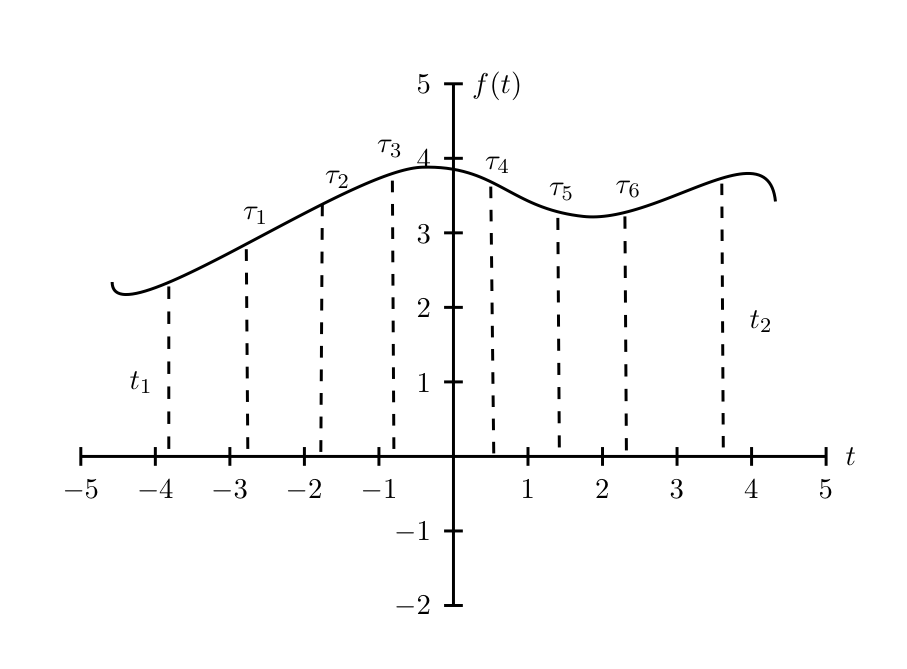
\includegraphics[scale=0.7]{Draw/function.png}
\label{}
\end{center}
\caption{Example for the integral of a function}
\label{function}
\end{figure}
Suppose that $f(t)$ represents the rate at which the size of the observable universe, $R(t)$, grows with time, that is to say $f(t)=\dot{R}(t)$; we wish to find how much the universe has expanded between $t_1$ and $t_2$, i.e. we want to calculate $R(t_2)-R(t_1)$, knowing $f(t)$ only. To do this, we must add up all the changes that $R(t)$ endures from time $t_1$ to time $t_2$: as a first approximation we break down the interval $t_2-t_1$ in several intermediate intervals $\{\tau_1,...,\tau_6\}$ and we perform the sum
\begin{equation}
R(t_2)-R(t_1)\approx f(t_1)(\tau_1-t_1)+f(\tau_1)(\tau_2-\tau_1)+...+f(\tau_6)(t_2-\tau_6)
\end{equation} 
What we are doing, basically, is approximating the area under the curve $f(t)$ enclosed by the horizontal axis and the two extremes $t_1$ and $t_2$; the above expression becomes exact when we the number of intermediate $\tau$ points that we choose becomes very large. This exact limit is called \textit{intergral} of the function $f(t)$ between $t_1$ and $t_2$ and is indicated by the notation
\begin{equation}
\int_{t_1}^{t_2}f(t)dt\equiv R(t_2)-R(t_1)
\end{equation}
This example also suggests us a statement, called \textit{fundamental theorem of calculus} that says that basically integrals and derivatives are one the inverse of the other; in fact, for \textit{any} function $R(t)$ it is true that
\begin{equation}
\int_{t_A}^{t_B}\dot{R}(t)dt=R(t_B)-R(t_A)
\end{equation}
That says that also the following is true
\begin{equation}
\frac{d}{dt}\int_{t_A}^t f(t')dt'=f(t)
\end{equation}
For \textit{any} function $f(t)$; a useful list of integrals of the most common functions can be found on \url{http://en.wikipedia.org/wiki/Lists_of_integrals}
\subsection{Differential equations}
The last concept that we need to understand before going into physical matters, is the one of \textit{differential equation}; the motivation of this is that nearly all physics is formulated in terms of statements of the kind ''we have this physical process, that causes this effect''. For example you may be already familiar with statements like ''we apply a force to a body and this causes the body to accelerate'' (the so called $F=ma$) or ''there is a temperature difference between two objects and this causes a heat flow''; you may notice that all these kinds of \textit{physical laws} can be written down in mathematical form, a form that looks like this 
\begin{equation}
\label{concept}
\mathrm{Effect(acceleration,heat \,flow)}=\mathrm{Cause(force,temperature \,difference)}
\end{equation} 
Usually the ``effect'' is the rate of change of some quantity (position, temperature,...) that involves derivatives, and the cause is some physical quantity that can depend on space and time (force for example): this is why these kind of physical laws are usually expressed in terms of \textit{differential equations} (i.e. equations that have a function as an unknown and relate the function itself to its derivatives). 
\subsubsection{Example 1}
A raindrop of mass $m$ originates from a cloud and starts falling to the ground; the forces acting on it are the usual gravity $mg$ and a frictional force that opposes to its motion. We suppose that this force is proportional to the velocity of the raindrop and write $F_{friction}=bv$ where $v$ is the vertical velocity of the raindrop. The addition of these two forces causes an acceleration, and we can write equation (\ref{concept}) as
\begin{equation}
ma=F_{gravity}-F_{friction}
\end{equation}
Or
\begin{equation}
\frac{dv(t)}{dt}=g-\frac{b}{m}v(t)
\end{equation}
We want to solve this equation for the time dependence of the velocity $v(t)$ and you can convince yourselves (looking at the derivative tables) that the solution is given by (assuming that the droplet is still at $t=0$):  
\begin{equation}
v(t)=\frac{mg}{b}(1-e^{-bt/m})
\end{equation}
\subsubsection{Example 2}
Consider a metal rod of length $L$ extending from $x=0$ to $x=L$; we keep its extremes in contact with some thermal bath so that their temperature is fixed $T(0)\equiv T_1$ and $T(L)\equiv T_2$; we want to find how the temperature of the rod changes along its length, that is to say we wish to find the function $T(x,t)$, which in general can also depend on time $t$. The physical law of heat conduction tells us that the temperature difference between points of the stick (expressed by its second derivative with respect to $x$, $\frac{\partial^2 T}{\partial x^2}$) \textit{has the effect} of causing a heat flow, expressed by the change of the temperature of the rod over time $\frac{\partial T}{\partial t}$. We may write the law of heat conduction as (take this for granted, we won't go into the details on why this is true)
\begin{equation}
\frac{\partial T(x,t)}{\partial t}=\frac{\partial^2 T(x,t)}{\partial x^2}
\end{equation} 
We seek for a \textit{stationary} solution to this equation (a solution that does not depend on time $T(x,t)=T(x)$) keeping in mind that we want to find the equilibrium profile $T(x)$; we try to solve 
\begin{equation}
\frac{d^2T(x)}{dx^2}=0
\end{equation}
Looking at the derivative table you can convince yourselves that the solution to this is given by $T(x)=ax+b$, with $a,b$ constants; for our particular problem of the rod this becomes 
\begin{equation}
T(x)=T_1+(T_2-T_1)\frac{x}{L}
\end{equation}
This completes a qualitative overview of the basic matematical instruments we need to understand (and give a justification) the most characteristic and intriguing aspects of Modern Cosmology; before going into the subject though, let us review the foundations and give a brief overview of classical physics and Newton's laws 

\section{Newton's laws}
All classical physics' phenomena (\textit{classical} means that neither quantum mechanics nor Einstein's relativity are involved in a significant way) can be described starting from these three assumptions, which were originally formulated by Isacc Newton in 17th century (backed up with the so called ''law zero'' which is an assumption on absolute space and time made by Galileo Galilei)
\begin{enumerate}
\setcounter{enumi}{-1}
\item \textit{Law zero}: there exist a special reference frame, which acts as an \textit{absolute} standard for space and time; the speed of light, $c$, is measured in this particular reference frame 
\item \textit{Law of inertia}: any physical body which experiences a \textit{zero net force} (i.e. a the sum of all forces acting on it is zero), $\mathbf{F}=0$, moves with a constant velocity $\dot{\mathbf{v}}=0$
\item \textit{Law of dynamics}: any physical body of mass $m$ that experiences a net force $\mathbf{F}$ will accelerate, with acceleration $\mathbf{a}$ given by $\mathbf{F}=m\mathbf{a}$
\item \textit{Law of action and reaction}: take two bodies labelled by $1,2$; suppose the first body exerts a force $\mathbf{F}_{12}$ on the second one. Then the second body as well exerts a force $\mathbf{F}_{21}$ on the first one, and these two forces are equal and opposite $\mathbf{F}_{21}=-\mathbf{F}_{12}$ 
\end{enumerate} 
Remember that all the quantities indicated in bold are \textit{vectors} in the sense discussed before; in order to have a taste on how these laws work, let us make some clarifying examples
\subsection{Gravity on earth's surface}
Consider an apple of mass $m$ which initially hangs from a tree at a height $z_0$ from the ground; at a certain instant ($t=0$) the apple starts to fall. We want to find how much time it will take to reach the ground; the gravitational force acting on it is $\mathbf{F}_g=-mg\hat{z}$ with $g$ being the gravitational acceleration at the earth surface, which is measured to be $g=9.81$\,m/s$^2$. Newton's second law tells us
\begin{equation}
\frac{d^2z(t)}{dt^2}=-g
\end{equation}
Which has the solution $z(t)=z_0-\frac{1}{2}gt^2$, and tells us that the apple will reach the ground in a time $T=\sqrt{\frac{2z_0}{g}}$
\subsection{Harmonic motion}
A block of mass $m$ is attached to a wall by means of a spring; we suppose that, when the block is pulled (or pushed) at a position $x$ from its equilibrium position (which corresponds to the spring rest length), it experiences a force $F=-kx$ with $k$ some constant. Let's define for convenience the \textit{angular frequency} $\omega$ as $k=m\omega^2$; again, Newton's second law tells us
\begin{equation}
\label{simpleharmonic}
\frac{d^2x(t)}{dt^2}=-\omega^2 x(t)
\end{equation}
This equation is more difficult to solve than the one in the previous problem, but the derivative tables help us again and we can find a general solution $x(t)=A\cos{\omega t}+B\sin{\omega t}$; if we let the initial conditions be $x(0)=x_0$ and $\dot{x}(0)=v(0)=v_0$ we immediately get
\begin{equation}
x(t)=x_0\cos{\omega t} + \frac{v_0}{\omega}\sin{\omega t}
\end{equation}
\subsection{Circular motion}
A little toy car of mass $m$ runs on a circular track of radius $R$ with constant speed $v$; despite the fact that the magnitude of the velocity $v$ is constant in this case, its direction is not and hence $\dot{\mathbf{v}}\neq 0$ and the car experiences acceleration and hence a net force from the track. Let's try to quantify this force; let $\hat{\mathbf{r}}$ be a unit vector that points in the car direction and $\hat{\theta}$ another unit vector that points along the car velocity, as in Figure \ref{track}; note that $\hat{\mathbf{r}}\cdot \hat{\theta}=0$. 
\begin{figure}
\begin{center}
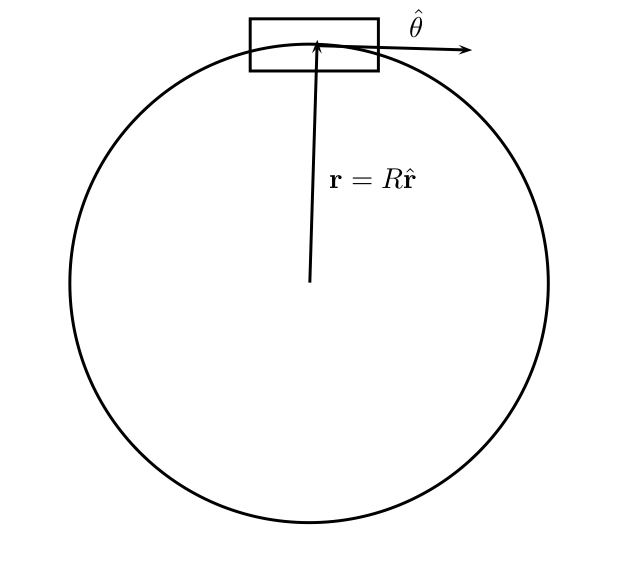
\includegraphics[scale=0.7]{Draw/circular.png}
\label{}
\end{center}
\caption{A toy car on a circular track}
\label{track}
\end{figure}
The position of the car is then described by the vector $\mathbf{r}=R\hat{\mathbf{r}}$; if we define the angular velocity of the car as $\omega=v/R$, assuming the following relations 
\begin{equation}
\frac{d}{dt}\hat{\mathbf{r}}(t)=\omega \hat{\theta}(t) \,\, ; \,\, \frac{d}{dt}\hat{\theta}(t)=-\omega \hat{\mathbf{r}}(t)
\end{equation}
We can find the acceleration of the car as
\begin{equation}
\label{centripetal}
\mathbf{a}(t)=\frac{d^2}{dt^2}\mathbf{r}(t)=R\frac{d}{dt}(\omega \hat{\theta}(t))=-\omega^2R\hat{\mathbf{r}}(t)=-a_c\hat{\mathbf{r}}(t) 
\end{equation}
Hence the car experiences an acceleration directed toward the center of the track, of magnitude $a_c=\omega^2R=v^2/R$, and hence a force directed toward the center of the track, of magnitude $F_c=m\omega^2 R=mv^2/R$.